\documentclass[a4paper]{article}

\usepackage{pgfplots}

\begin{document}

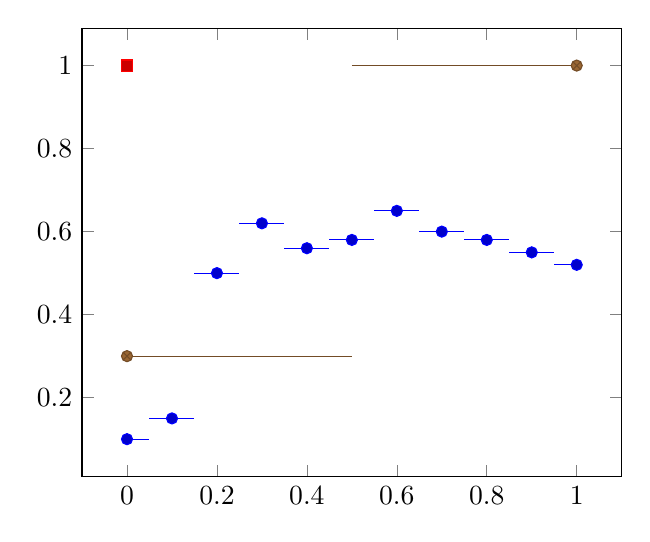
\begin{tikzpicture}
\begin{axis}
\addplot+[jump mark mid]
coordinates
{(0,0.1)    (0.1,0.15) (0.2,0.5)  (0.3,0.62)
 (0.4,0.56) (0.5,0.58) (0.6,0.65) (0.7,0.6)
 (0.8,0.58) (0.9,0.55) (1,0.52)};

\addplot+[jump mark mid]
coordinates
{(0,1)    };

\addplot+[jump mark mid]
coordinates
{(0,0.3) (1,1)    };
\end{axis}
\end{tikzpicture}

\begin{tikzpicture}
\begin{axis}
\addplot+[jump mark mid]
coordinates
{(0,0.1)    (0.1,0.15) (0.3,0.62)
 (0.4,0.56) (0.5,0.58) (0.7,0.6)
 (0.8,0.58) (0.9,0.55) (1,0.52)};
\end{axis}
\end{tikzpicture}

\end{document}

